\documentclass{jlreq}

\usepackage{mystyle,tikz,autonum,mathtools}
\usetikzlibrary{calc}

%\newcommand{\pt}[1]{\mathrm{#1}}
\newcommand{\Norm}[1]{\lvert #1 \rvert}

\DeclarePairedDelimiterX{\SetComprehension}[2]{\{}{\}}{\, #1 \mathopen{}\,\delimsize|\,\mathopen{} #2 \,}

\title{2018年度京都大学文系数学第4問}
\author{オ}
\date{\today}

\begin{document}
	
	\maketitle
	
	\begin{abstract}
		解きました.
	\end{abstract}
	
	\begin{question}
		四面体$\mathrm{ABCD}$は$\mathrm{AC} = \mathrm{BD},\, \mathrm{AD} = \mathrm{BC}$を満たすとし,
		辺$\mathrm{AB}$の中点を$\mathrm{P}$,
		辺$\mathrm{CD}$の中点を$\mathrm{Q}$とする.
		\begin{enumerate}[label=(\arabic*)\ ]
			\item 辺$\mathrm{AB}$と線分$\mathrm{PQ}$は垂直であることを示せ.
			\item 線分$\mathrm{PQ}$を含む平面$\alpha$で四面体$\mathrm{ABCD}$を切って2つの部分に分ける.
			このとき,
			2つの部分の体積は等しいことを示せ.
		\end{enumerate}
	\end{question}
	
	\begin{enumerate}[label=(\arabic*)\ ]
		\item $b = \overrightarrow{\mathrm{AB}},\, c = \overrightarrow{\mathrm{AC}},\, d = \overrightarrow{\mathrm{AD}}$と置く\footnote{矢印をつけるべきだろうけど面倒なので省略する.}.
		\begin{equation}
			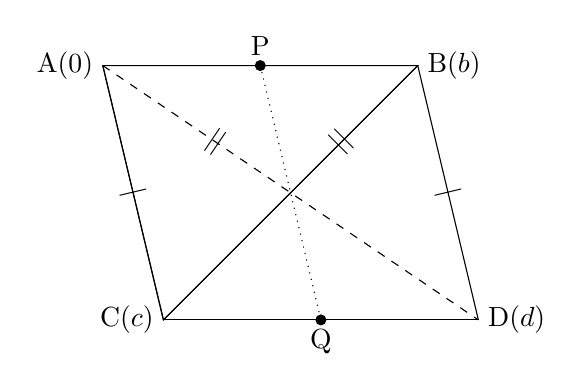
\begin{tikzpicture}
				\renewcommand{\k}{0.3}
				\begin{scope}[scale=2]
					% 定義
					\coordinate (A) at (0, 0, 0);
					\coordinate (B) at (2, 0, 0);
					\coordinate (C) at (0, -2, -1);
					\coordinate (D) at (2, -2, -1);
					\coordinate (P) at ($(A)!0.5!(B)$);
					\coordinate (Q) at ($(C)!0.5!(D)$);
					\coordinate (R) at ($(A)!\k!(C)$);
					\coordinate (S) at ($(B)!\k!(D)$);
				\end{scope}
				
				% 辺の描画
				\draw (A) -- (B) -- (C) -- cycle; % 底面ABC
				\draw (A) -- node[sloped] {$|$} (C);
				\draw[dashed] (A) -- node[sloped,pos=0.3] {$||$} (D);
				\draw (B) -- node[sloped] {$|$} (D);
				\draw (C) -- (D);
				\draw (B) -- node[sloped,pos=0.3] {$||$} (C);
				%			\draw[dotted] (P) -- (S);
				%			\draw[dotted] (R) -- (Q);
				%			\draw (P) -- (R);
				%			\draw (S) -- (Q);
				
							\draw[dotted] (P) -- (Q);
				
				%			\draw (A) -- node[sloped] {$\circ$} (R);
				%			\draw (B) -- node[sloped] {$\circ$} (S);
				
				% 頂点のラベル
				\node at (A) [left] {$\mathrm{A}(0)$};
				\node at (B) [right] {$\mathrm{B}(b)$};
				\node at (C) [left] {$\mathrm{C}(c)$};
				\node at (D) [right] {$\mathrm{D}(d)$};
				
				\fill (P) node[above] {P} circle[radius=.07];
				\fill (Q) node[below] {Q} circle[radius=.07];
				%			\fill (R) node[left] {R} circle[radius=.07];
				%			\fill (S) node[right] {S} circle[radius=.07];
			\end{tikzpicture}
		\end{equation}
		このとき,
		$\mathrm{AC} = \mathrm{BD}$より
		\begin{align}
			\Norm{d - b}^2 - \Norm{c}^2
			&= \Norm{b}^2 - 2 b \cdot d + \Norm{d}^2 - \Norm{c}^2 \\
			&= 0
		\end{align}
		だから,
		\begin{equation}
			b \cdot d
			= \frac{\Norm{b}^2 - \Norm{c}^2 + \Norm{d}^2}{2}
		\end{equation}
		が分かる.
		同様にして,
		$\mathrm{AD} = \mathrm{BC}$より
		\begin{equation}
			b \cdot c
			= \frac{\Norm{b}^2 + \Norm{c}^2 - \Norm{d}^2}{2}
		\end{equation}
		を得る.
		したがって,
		\begin{align}
			\overrightarrow{\mathrm{AB}} \cdot \overrightarrow{\mathrm{PQ}}
			&= b \cdot \left(\frac{1}{2} c + \frac{1}{2} d - \frac{1}{2} b\right) \\
			&= \frac{1}{2} \left(\frac{\Norm{b}^2 + \Norm{c}^2 - \Norm{d}^2}{2} + \frac{\Norm{b}^2 - \Norm{c}^2 + \Norm{d}^2}{2} - \Norm{b}^2\right) \\
			&= 0
		\end{align}
		だから,
		$\mathrm{AB} \perp \mathrm{PQ}$である.
		\item Rを辺ACまたは辺AD上の点とし,
		$r = \overrightarrow{\mathrm{AR}}$と置く.
		平面$\alpha$は3点$\mathrm{P}, \mathrm{Q}, \mathrm{R}$を含む平面だとしてもよい\footnote{面ACD上に,
		点Qを中心とした半円周Oを考える.
		平面$\alpha$と$\mathrm{O} \setminus \{\mathrm{D}\}$のただ一つの交点を$\mathrm{R}'$と置けば,
		$\alpha$と$\mathrm{R}'$は1対1に対応する.
		直線$\mathrm{QR}'$は辺ACまたは,
		辺ADから点Dを除いた部分と交わるので,
		その交点をRと置く.
		Rと$\mathrm{R}'$は1対1に対応し,
		$\alpha$はP, Q, Rを含む.}
		
		\begin{itemize}
			\item[($\mathrm{R} = \mathrm{A}$のとき)] 分けられた部分同士は平面$\alpha$に関して対称なので,
			それらの体積は一致する.
			\begin{equation}
				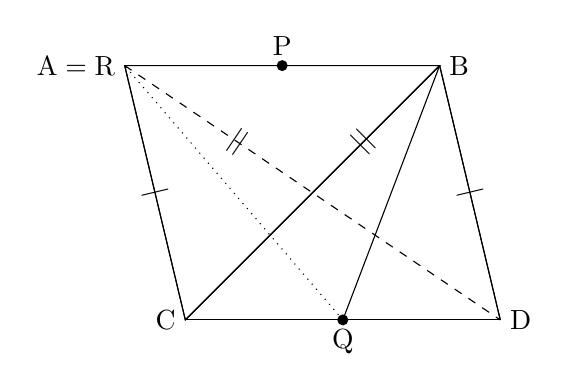
\begin{tikzpicture}
					\renewcommand{\k}{0.3}
					\begin{scope}[scale=2]
						% 定義
						\coordinate (A) at (0, 0, 0);
						\coordinate (B) at (2, 0, 0);
						\coordinate (C) at (0, -2, -1);
						\coordinate (D) at (2, -2, -1);
						\coordinate (P) at ($(A)!0.5!(B)$);
						\coordinate (Q) at ($(C)!0.5!(D)$);
						\coordinate (R) at (A);
						\coordinate (S) at ($(B)!\k!(D)$);
					\end{scope}
					
					% 辺の描画
					\draw (A) -- (B) -- (C) -- cycle; % 底面ABC
					\draw (R) -- node[sloped] {$|$} (C);
					\draw[dashed] (A) -- node[sloped,pos=0.3] {$||$} (D);
					\draw (B) -- node[sloped] {$|$} (D);
					\draw (C) -- (D);
					\draw (B) -- node[sloped,pos=0.3] {$||$} (C);
%					\draw[dotted] (P) -- (S);
%					\draw[dotted] (R) -- (Q);
%					\draw (P) -- (R);
%					\draw (S) -- (Q);
					\draw (B) -- (D);
					\draw[dotted] (Q) -- (A);
					\draw (B) -- (Q);
					
					%			\draw[dotted] (P) -- (Q);
					
%					\draw (A) -- node[sloped] {$\circ$} (R);
%					\draw (B) -- node[sloped] {$\circ$} (S);
					
					% 頂点のラベル
					\node at (A) [left] {$\mathrm{A} = \mathrm{R}$};
					\node at (B) [right] {B};
					\node at (C) [left] {C};
					\node at (D) [right] {D};
					
					\fill (P) node[above] {P} circle[radius=.07];
					\fill (Q) node[below] {Q} circle[radius=.07];
%					\fill (R) node[left] {R} circle[radius=.07];
%					\fill (S) node[right] {S} circle[radius=.07];
				\end{tikzpicture}
			\end{equation}
			\item[(Rが辺ACから点Aを除いた部分上にあるとき)\ ] $r = k c\ (0 \le k \le 1)$とできる.
			このとき,
			\begin{align}
				\alpha
				&= \SetComprehension{u p + v q + w r}{u + v + w = 1} \\
				&= \SetComprehension*{\frac{u}{2} b + \left(\frac{v}{2} + w k\right) c + \frac{v}{2} d}{u + v + w = 1}
			\end{align}
			である.
			$\alpha$と辺BDの交点をSとし,
			$s = \overrightarrow{\mathrm{AS}}$と置く.
			$s = l b + (1 - l) d\ (0 \le l \le 1)$とすれば,
			$s \in \alpha$なので
			\begin{equation}
				\begin{cases}
					\dfrac{u}{2} = l \\
					\dfrac{v}{2} + w k = 0 \\
					\dfrac{v}{2} = 1 - l
				\end{cases}
			\end{equation}
			を得る.
			$u + v + w = 1$より
			\begin{equation}
				2 l + 2 (1 - l) - \frac{2 (1 - l)}{2 k} = 1
			\end{equation}
			なので,
			$l = 1 - k$が分かる.
			したがって,
			点Sは辺BDを$k : (1 - k)$に内分する.
			\begin{equation}
				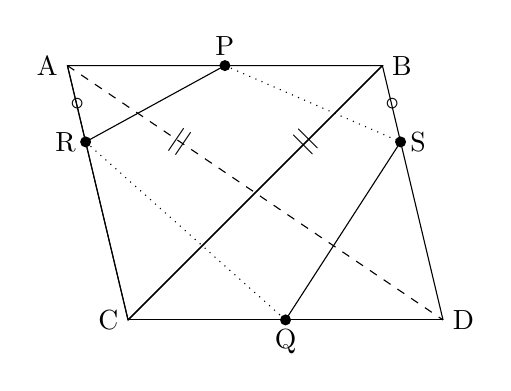
\begin{tikzpicture}
					\renewcommand{\k}{0.3}
					\begin{scope}[scale=2]
						% 定義
						\coordinate (A) at (0, 0, 0);
						\coordinate (B) at (2, 0, 0);
						\coordinate (C) at (0, -2, -1);
						\coordinate (D) at (2, -2, -1);
						\coordinate (P) at ($(A)!0.5!(B)$);
						\coordinate (Q) at ($(C)!0.5!(D)$);
						\coordinate (R) at ($(A)!\k!(C)$);
						\coordinate (S) at ($(B)!\k!(D)$);
					\end{scope}
					
					% 辺の描画
					\draw (A) -- (B) -- (C) -- cycle; % 底面ABC
					\draw (R) -- node[sloped] {$\square$} (C);
					\draw[dashed] (A) -- node[sloped,pos=0.3] {$||$} (D);
					\draw (S) -- node[sloped] {$\square$} (D);
					\draw (C) -- (D);
					\draw (B) -- node[sloped,pos=0.3] {$||$} (C);
					\draw[dotted] (P) -- (S);
					\draw[dotted] (R) -- (Q);
					\draw (P) -- (R);
					\draw (S) -- (Q);
					
					%			\draw[dotted] (P) -- (Q);
					
					\draw (A) -- node[sloped] {$\circ$} (R);
					\draw (B) -- node[sloped] {$\circ$} (S);
					
					% 頂点のラベル
					\node at (A) [left] {A};
					\node at (B) [right] {B};
					\node at (C) [left] {C};
					\node at (D) [right] {D};
					
					\fill (P) node[above] {P} circle[radius=.07];
					\fill (Q) node[below] {Q} circle[radius=.07];
					\fill (R) node[left] {R} circle[radius=.07];
					\fill (S) node[right] {S} circle[radius=.07];
				\end{tikzpicture}
			\end{equation}
			$\triangle \mathrm{ABC} \equiv \triangle \mathrm{BAD}$と$\triangle \mathrm{ACD} \equiv \triangle \mathrm{BDC}$より,
			$\mathrm{PR} = \mathrm{PS}$と$\mathrm{QR} = \mathrm{QS}$が分かる.
			よって.
			立体APR-DQSと立体BPS-CQRは回転と平行移動によって一致する.
			\begin{equation}
				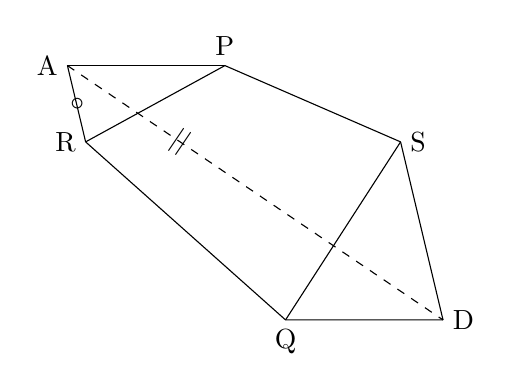
\begin{tikzpicture}
					\renewcommand{\k}{0.3}
					\begin{scope}[scale=2]
						% 定義
						\coordinate (A) at (0, 0, 0);
						\coordinate (B) at (2, 0, 0);
						\coordinate (C) at (0, -2, -1);
						\coordinate (D) at (2, -2, -1);
						\coordinate (P) at ($(A)!0.5!(B)$);
						\coordinate (Q) at ($(C)!0.5!(D)$);
						\coordinate (R) at ($(A)!\k!(C)$);
						\coordinate (S) at ($(B)!\k!(D)$);
					\end{scope}
					
					% 辺の描画
%					\draw (A) -- (B) -- (C) -- cycle; % 底面ABC
%					\draw (R) -- node[sloped] {$\square$} (C);
					\draw[dashed] (A) -- node[sloped,pos=0.3] {$||$} (D);
					\draw (S) -- node[sloped] {$\square$} (D);
%					\draw (C) -- (D);
%					\draw (B) -- node[sloped,pos=0.3] {$||$} (C);
					\draw (P) -- (S);
					\draw (R) -- (Q) -- (D);
					\draw (P) -- (R);
					\draw (S) -- (Q);
					\draw (A) -- (P);
					
					%			\draw[dotted] (P) -- (Q);
					
					\draw (A) -- node[sloped] {$\circ$} (R);
%					\draw (B) -- node[sloped] {$\circ$} (S);
					
					% 頂点のラベル
					\node at (A) [left] {A};
%					\node at (B) [right] {B};
%					\node at (C) [left] {C};
					\node at (D) [right] {D};
					
					\fill (P) node[above] {P} ;
					\fill (Q) node[below] {Q} ;
					\fill (R) node[left] {R} ;
					\fill (S) node[right] {S} ;
				\end{tikzpicture}
				\qquad
				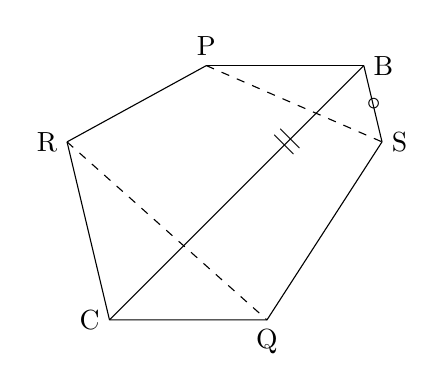
\begin{tikzpicture}
					\renewcommand{\k}{0.3}
					\begin{scope}[scale=2]
						% 定義
						\coordinate (A) at (0, 0, 0);
						\coordinate (B) at (2, 0, 0);
						\coordinate (C) at (0, -2, -1);
						\coordinate (D) at (2, -2, -1);
						\coordinate (P) at ($(A)!0.5!(B)$);
						\coordinate (Q) at ($(C)!0.5!(D)$);
						\coordinate (R) at ($(A)!\k!(C)$);
						\coordinate (S) at ($(B)!\k!(D)$);
					\end{scope}
					
					% 辺の描画
%					\draw (A) -- (B) -- (C) -- cycle; % 底面ABC
					\draw (R) -- node[sloped] {$\square$} (C);
%					\draw[dashed] (A) -- node[sloped,pos=0.3] {$||$} (D);
%					\draw (S) -- node[sloped] {$\square$} (D);
%					\draw (C) -- (D);
					\draw (B) -- node[sloped,pos=0.3] {$||$} (C);
					\draw[dashed] (P) -- (S);
					\draw[dashed] (R) -- (Q);
					\draw (P) -- (R);
					\draw (S) -- (Q) -- (C);
					\draw (P) -- (B);
					
					%			\draw[dotted] (P) -- (Q);
					
%					\draw (A) -- node[sloped] {$\circ$} (R);
					\draw (B) -- node[sloped] {$\circ$} (S);
					
					% 頂点のラベル
%					\node at (A) [left] {A};
					\node at (B) [right] {B};
					\node at (C) [left] {C};
%					\node at (D) [right] {D};
					
					\fill (P) node[above] {P} ;
					\fill (Q) node[below] {Q} ;
					\fill (R) node[left] {R} ;
					\fill (S) node[right] {S} ;
				\end{tikzpicture}
			\end{equation}
			よって,
			これらの体積も一致する.
			\item[(Rが辺ADから点Aを除いた部分上にあるとき)\ ] 点Cと点Dを入れ替えた四面体を考えれば,
			Rが辺AC上にある場合に帰着する.
		\end{itemize}
		以上より,
		PQを含むいかなる平面$\alpha$に対しても,
		2つの部分の体積は一致する.
	\end{enumerate}
	
%	\begin{equation}
%		\begin{tikzpicture}
%			\renewcommand{\k}{0.3}
%			\begin{scope}[scale=2]
%				% 定義
%				\coordinate (A) at (0, 0, 0);
%				\coordinate (B) at (2, 0, 0);
%				\coordinate (C) at (0, -2, -1);
%				\coordinate (D) at (2, -2, -1);
%				\coordinate (P) at ($(A)!0.5!(B)$);
%				\coordinate (Q) at ($(C)!0.5!(D)$);
%				\coordinate (R) at ($(A)!\k!(C)$);
%				\coordinate (S) at ($(B)!\k!(D)$);
%			\end{scope}
%			
%			% 辺の描画
%			\draw (A) -- (B) -- (C) -- cycle; % 底面ABC
%			\draw (A) -- node[sloped] {$|$} (C);
%			\draw[dashed] (A) -- node[sloped,pos=0.3] {$||$} (D);
%			\draw (B) -- node[sloped] {$|$} (D);
%			\draw (C) -- (D);
%			\draw (B) -- node[sloped,pos=0.3] {$||$} (C);
%%			\draw[dotted] (P) -- (S);
%%			\draw[dotted] (R) -- (Q);
%%			\draw (P) -- (R);
%%			\draw (S) -- (Q);
%			
%%			\draw[dotted] (P) -- (Q);
%			
%%			\draw (A) -- node[sloped] {$\circ$} (R);
%%			\draw (B) -- node[sloped] {$\circ$} (S);
%			
%			% 頂点のラベル
%			\node at (A) [left] {A};
%			\node at (B) [right] {B};
%			\node at (C) [left] {C};
%			\node at (D) [right] {D};
%			
%			\fill (P) node[above] {P} circle[radius=.07];
%			\fill (Q) node[below] {Q} circle[radius=.07];
%%			\fill (R) node[left] {R} circle[radius=.07];
%%			\fill (S) node[right] {S} circle[radius=.07];
%		\end{tikzpicture}
%	\end{equation}
	
\end{document}